\chapter{Evaluation}
\label{cha:evaluation}
In this chapter we present the evaluation of the work done. This will measure the performance and scalability of the integration by presenting benchmarks of the running system.\par
	Section \ref{sec:operation_propagation_time} will measure how the number of operation each message contains influences the time needed to propagate them. In section \ref{sec:meta-data_size} will be shown how the meta-data stored in Antidote increases with the operations executed in the system.

\section{Operation Propagation Time}
\label{sec:operation_propagation_time}
In this section we will focus on measuring the propagation time of system operations and how it fluctuates with other variables. In this test scenario, we use one Antidote instance, one legion object server instance, one Antidote client and one Legion node. This experiment consists in saving the current time in one client, when the update is issued. The update is sent and when the other client detects to have received the update, saves the time and finally makes the difference between the two times.\par
	Firstly, in figure \ref{graph1} we measure the operation propagation time scaling with the number of operations in each message. As we can see, the time it takes to propagate a message, increases with the number of operations that each message contains. When propagating messages from Legion to Antidote, the time required increases nearly linearly with the number of operations. On the other hand, when propagating messages from Antidote to legion, the time required does not grow as fast, only increasing slightly with the number of operations in each message.

\begin{figure}[H]
\centering
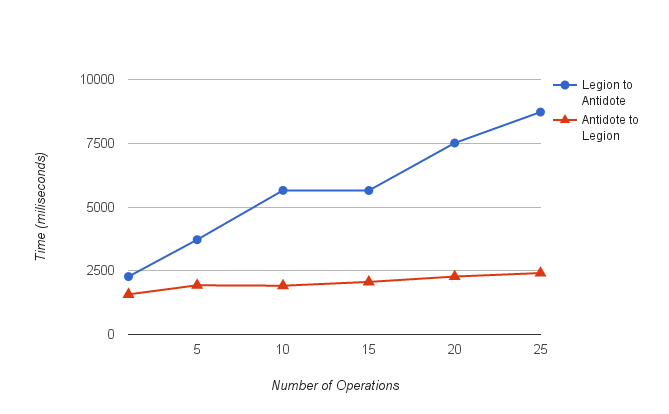
\includegraphics[scale=0.7]{files/graph1.png}
\caption{Propagation time scaling with operation per message}
\label{graph1}
\end{figure}

Secondly, in CENAS we  measure the scalability of the message propagation time with the size of the message. As we can see, the time needed to propagate a message does not seem to scale with the size of the message, this applies for the two update directions.

\section{Meta-Data Size}
\label{sec:meta-data_size}